\section{Introduction}
Program synthesis (or code generation) is a long-standing problem explored since the early days of computer science~\cite{manna1971toward}. 
Recently, instruction tuning of code \llmfull{s} (\llm{s}) has been used to improve many coding tasks~\cite{codealpaca, luo2023wizardcoder, wei2023magicoder}, such as text-to-code generation~\cite{chen2021evaluating, austin2021program}, code completion~\cite{cassano2022multiple}, and data science engineering~\cite{lai2022ds1000}. 

\begin{figure}[t]
\centering
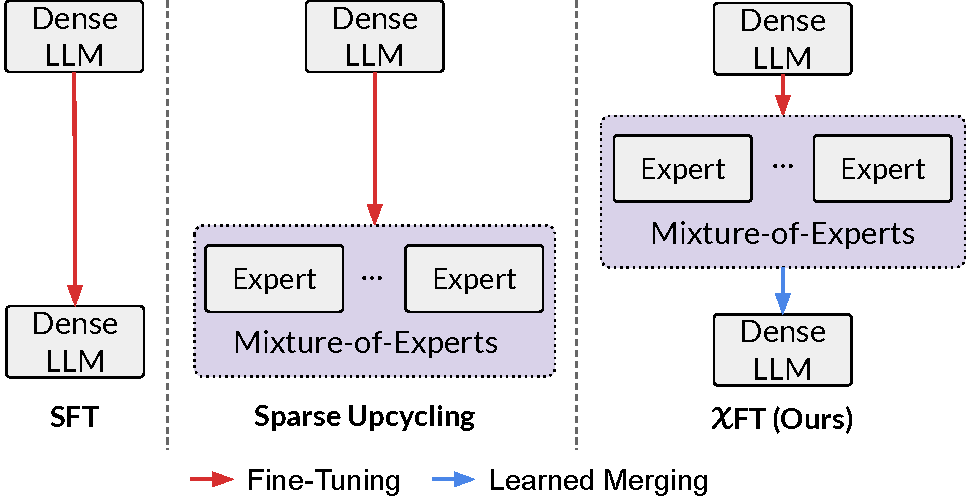
\includegraphics[width=1.0\linewidth]{assets/comparison.pdf}
\caption{Overview of SFT, \sparseupcycle, and \ours.}
\label{fig:comparison}
\end{figure}

A typical instruction tuning flow involves two steps~\cite{zhang2023instruction}: 
(i) curating an instruction dataset of instruction-output pairs, where the instruction reflects human intents in natural language and the output includes explained code snippets that correspond to the intent; 
and 
(ii) supervised fine-tuning of pre-trained \llm on the instruction dataset. 
In the realm of code, multiple instruction-tuning methods have been proposed to curate high-quality instruction datasets.
For example, \textit{Code \evolinstruct}~\cite{luo2023wizardcoder} uses \chatgpt to obtain complex synthetic code instructions with heuristic prompts, while \ossinstruct~\cite{wei2023magicoder} prompts \chatgpt to generate new coding problems by drawing inspiration from open source code snippets.
While existing work focuses on the data perspectives of instruction tuning, 
they all follow the standard SFT, leaving room for exploring advanced training schemes.




We argue that prior works largely overlook the possibility of improving the code instruction tuning by advancing the training schemes.
Figure~\ref{fig:comparison} depicts the supervised fine-tuning (SFT), which directly starts with the pre-trained weights and architecture for fine-tuning.
The model is \emph{dense} here because all parameters are activated to compute the next token (assuming it is a decoder-only \llm{}).
In contrast to fine-tuning a \emph{dense} model, 
following the scaling laws~\cite{kaplan2020scaling} (\ie more parameters, better performance),
\sparseupcycle~\cite{komatsuzaki2023sparse} is proposed to efficiently upgrade the model sizes by upcycling a dense \llm to a sparsely activated \moefull (\moe) model.
An \moe model is efficient because the generation of the next token only involves a subset of parameters (\ie experts) and thus is \emph{sparsely activated}.
For example, Mixtral-8x7B~\cite{jiang2024mixtral}, compared to a dense 7B model, 
uses approximately $8\times$ parameters and $2\times$ computation, \ie only 2 out of 8 experts are dynamically selected to compute the next token.
However, there are two key limitations when using \sparseupcycle in instruction tuning:
(i) \emph{Slow scaling:} \citet{komatsuzaki2023sparse} show that \sparseupcycle improves the dense SFT marginally at the early phase, requiring orders of magnitude of extra compute to achieve decent improvement;
and (ii) \emph{Inference cost:}
though \moe is more efficient than directly scaling the size of dense \llm{s},
\moe is still expensive, especially at inference, 
as it introduces significantly more parameters (\ie memory) and, more importantly, computes during inference, compared to its dense counterparts.

In this paper, we propose \textbf{\ours}: 
by simply merging upcycled \moe models, we push the performance limit of instruction-tuned code \llm{s}.
While vanilla \sparseupcycle fails to improve instruction tuning efficiently~\cite{komatsuzaki2023sparse},
\ours addresses this challenge by isolating one expert as the shared expert among all the other experts in each \moe layer, inspired by \deepseekmoe~\cite{dai2024deepseekmoe} and \mocle~\cite{gou2024mixture}.
\ours also includes a novel routing weight normalization strategy to eliminate scale mismatch between the upcycled \moe layer with the shared expert and the original dense layer, which will otherwise lead to performance degradation~\cite{wu2022residual}. 
After the upcycled \moe model finishes the SFT phase, motivated by \modelsoup~\cite{wortsman2022model}, 
\ours uses a learnable model merging mechanism to output a dense model by merging all the expert networks in the upcycled \moe, 
\ie the final dense model is of the same model structure and size as the original pre-trained model,
achieving similar performance without paying extra inference cost as the \sparseupcycle.
With only 1.3B parameters, \ours achieves 67.1 \passat{1} on \humaneval and 64.6 \passat{1} on \humanevalp, which is the new state-of-the-art for tiny code \llm{s} (<3B).
Compared with SFT, \ours achieves 13\% improvement on \humanevalp.
Surprisingly, our model merging mechanism can preserve or even further boost the general performance of the upcycled \moe with around $\sfrac{1}{8}\times$ parameters! 
We conclude our contribution as follows:
\begin{itemize}[leftmargin=1em]
    \setlength{\parskip}{2pt}
    \setlength\itemsep{0pt}
    \item \textbf{Dimension:} 
    We open a new dimension of improving instruction tuning of code \llm{s} by advancing its training scheme, using enhanced \sparseupcycle and learnable model merging mechanism, which neither changes the final model structure nor requires more training data.
    \item \textbf{Technique:} 
    We present \ours, a new training scheme for code instruction tuning. \ours involves two steps: \emph{upcycling} and \emph{merging}. A pre-trained dense \llm is first upcycled into an \moe with the shared expert setting and then fine-tuned on the instruction dataset. To avoid the performance degradation caused by the scale mismatch issue,
    we propose a novel routing weight normalization strategy. In addition, we introduce the first learnable mechanism 
    for merging the upcycled \moe into a dense model, eliminating additional inference overhead while preserving or even improving the \moe performance.
    \item \textbf{Results:} With only 1.3B parameters, \ours achieves 67.1 \passat{1} on \humaneval and 64.6 \passat{1} on \humanevalp, which is the new state-of-the-art for tiny code \llm{s} (<3B). Compared with normal supervised fine-tuning (SFT), \ours achieves 13\% improvement on \humanevalp! \ours also achieves a consistent improvement from 2\% to 13\% on \mbpp, \multiple, and \dsonek over SFT, demonstrating its generalization.
\end{itemize}
